
%%%%%%%%%%%%%%%%%% PREAMBULE %%%%%%%%%%%%%%%%%%

\documentclass[aspectratio=169,utf8]{beamer}
%\documentclass[aspectratio=169,handout]{beamer}

\usetheme{Boadilla}
%\usecolortheme{seahorse}
%\usecolortheme[RGB={85,40,4}]{structure}
\usecolortheme[RGB={127,0,0}]{structure}
\useoutertheme{infolines}

% packages
\usepackage{amsfonts,amsmath,amssymb,amsthm}
\usepackage[utf8]{inputenc}
\usepackage[T1]{fontenc}
\usepackage{lmodern}

\usepackage[francais]{babel}
\usepackage{fancybox}
\usepackage{graphicx}


\usepackage{tikz}
\usetikzlibrary{shapes,snakes}


%\usepackage[usenames, x11names]{xcolor}


%\usepackage{mathptmx}
%\usepackage{fouriernc}
%\usepackage{newcent}
%\usepackage[mathcal,mathbf]{euler}

%\usepackage{palatino}
%\usepackage{newcent}
%\usepackage[mathcal,mathbf]{euler}


%----- Presentation ------
\setlength{\parindent}{0cm}

%\newcommand{\ExoSept}{\href{http://exo7.emath.fr}{\textbf{\textsf{Exo7}}}}

\definecolor{myred}{rgb}{0.93,0.26,0}
\definecolor{myorange}{rgb}{0.97,0.58,0}
\definecolor{myyellow}{rgb}{1,0.86,0}

\newcommand{\LogoExoSept}[1]{  % input : echelle
{\usefont{U}{cmss}{bx}{n}
\begin{tikzpicture}[scale=0.1*#1,transform shape]
  \fill[color=myorange] (0,0)--(4,0)--(4,-4)--(0,-4)--cycle;
  \fill[color=myred] (0,0)--(0,3)--(-3,3)--(-3,0)--cycle;
  \fill[color=myyellow] (4,0)--(7,4)--(3,7)--(0,3)--cycle;
  \node[scale=5] at (3.5,3.5) {Exo7};
\end{tikzpicture}}
}



% New command Arnaud -- november 2011
%\setbeamersize{text margin left=24ex}
% si vous modifier cette valeur il faut aussi
% modifier le decalage du titre pour compenser
% (ex : ici =+10ex, titre =-5ex



%--------------- Commande beamer---------------
\newcommand{\beameronly}[1]{#1} % permet de mettre des pause dans beamer pas dans poly


\setbeamertemplate{navigation symbols}{}
\setbeamertemplate{footline}  % tiré du fichier beamerouterinfolines.sty
{
  \leavevmode%
  \hbox{%
  \begin{beamercolorbox}[wd=.333333\paperwidth,ht=2.25ex,dp=1ex,center]{author in head/foot}%
    % \usebeamerfont{author in head/foot}\insertshortauthor%~~(\insertshortinstitute)
    \usebeamerfont{section in head/foot}{\bf\insertshorttitle}
  \end{beamercolorbox}%
  \begin{beamercolorbox}[wd=.333333\paperwidth,ht=2.25ex,dp=1ex,center]{title in head/foot}%
    \usebeamerfont{section in head/foot}{\bf\insertsectionhead}
  \end{beamercolorbox}%
  \begin{beamercolorbox}[wd=.333333\paperwidth,ht=2.25ex,dp=1ex,right]{date in head/foot}%
    % \usebeamerfont{date in head/foot}\insertshortdate{}\hspace*{2em}
 %   \insertframenumber{} / \inserttotalframenumber\hspace*{2ex} 
  \end{beamercolorbox}}%
  \vskip0pt%
}


\definecolor{mygrey}{rgb}{0.5,0.5,0.5}
\setlength{\parindent}{0cm}
%\DeclareTextFontCommand{\helvetica}{\fontfamily{phv}\selectfont}

% background beamer
\definecolor{couleurhaut}{rgb}{0.85,0.9,1}  % creme
\definecolor{couleurmilieu}{rgb}{1,1,1}  % vert pale
\definecolor{couleurbas}{rgb}{0.85,0.9,1}  % blanc
\setbeamertemplate{background canvas}[vertical shading]%
[top=couleurhaut,middle=couleurmilieu,midpoint=0.4,bottom=couleurbas] 
%[top=fondtitre!05,bottom=fondtitre!60]

%----------- Boite teaser ------------------




% Commande spécifique à ce chapitre



%%%%%%%%%%%%%%%%%%%%%%%%%%%%%%%%%%%%%%%%%%%%%%%%%%%%%%%%%%%%%
%%%%%%%%%%%%%%%%%%%%%%%%%%%%%%%%%%%%%%%%%%%%%%%%%%%%%%%%%%%%%


\begin{document}


\tikzstyle{mybox} = [draw=myred, fill=red!20, very thick,
    rectangle, rounded corners, inner sep=0pt, inner ysep=20pt]
\tikzstyle{fancytitle} =[fill=myred, text=white, ellipse]

\centering

\begin{frame}


\begin{tikzpicture}[scale = 1.5, transform shape, rotate=0, baseline=-3.5cm]
\node [mybox] (box) {%
    \begin{minipage}[t!]{0.4\textwidth}
\centering \bf En route pour la cryptographie
    \end{minipage}
    };
\node[fancytitle] at (box.north) {\bf \large Arithmétique};
\end{tikzpicture}

\vfill
\pause

\textbf{Un MOOC de l'université Lille 1}

\medskip


\includegraphics[scale=0.5]{Fig-crypto/logoLille1_transp.png} 

\medskip

\end{frame}


\begin{frame}
\begin{tikzpicture}[scale = 1, transform shape, rotate=0, baseline=-3.5cm]
\node [mybox] (box) {%
    \begin{minipage}[t!]{0.4\textwidth}
\centering \bf En route pour la cryptographie
    \end{minipage}
    };
\node[fancytitle] at (box.north) {\bf \large Arithmétique};
\end{tikzpicture}



\vspace*{-20mm}

\begin{tabular}{c}
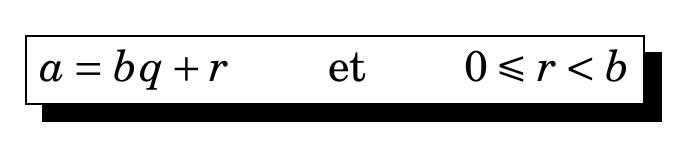
\includegraphics[scale=0.20]{Fig-crypto/img-division.png} \\
\pause
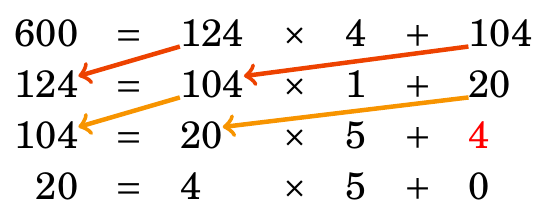
\includegraphics[scale=0.2]{Fig-crypto/img-pgcd.png} \\
\pause
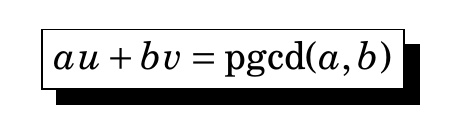
\includegraphics[scale=0.25]{Fig-crypto/img-bezout.png} \\
\pause
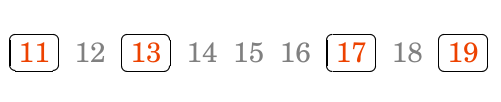
\includegraphics[scale=0.25]{Fig-crypto/img-premiers.png} \\ 
\end{tabular}

\end{frame}

\begin{frame}
\begin{tikzpicture}[scale = 1, transform shape, rotate=0, baseline=-3.5cm]
\node [mybox] (box) {%
    \begin{minipage}[t!]{0.4\textwidth}
\centering \bf En route pour la cryptographie
    \end{minipage}
    };
\node[fancytitle] at (box.north) {\bf \large Arithmétique};
\end{tikzpicture}



\vspace*{-20mm}

\begin{tabular}{cc}
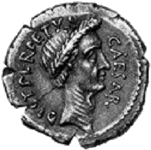
\includegraphics[scale=0.4]{Fig-crypto/week1-cesar_transp.png} &
\pause
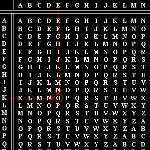
\includegraphics[scale=0.45]{Fig-crypto/week2-vigenere.png} \\
\pause
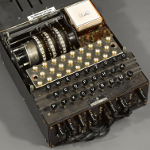
\includegraphics[scale=0.4]{Fig-crypto/week3-enigma.png} &
\pause

\includegraphics[scale=0.8]{Fig-crypto/cadena.png} \\ 
\end{tabular}


% \Large
% \begin{itemize}
%   \item Arithmétique
%   \begin{itemize}
%     \item Division euclidienne
%     \item Modulo
%     \item pgcd 
%     \item Théorème de Bézout
%     \item Nombres premiers
%   \end{itemize}
%   \item Cryptographie
%   \begin{itemize}
%     \item Le code de César
%     \item Le chiffre de Vigenère
%     \item La machine Enigma
%     \item Le code RSA
%   \end{itemize}
% \end{itemize}

\end{frame}

% \begin{frame}
% \begin{tikzpicture}[scale = 1, transform shape, rotate=0, baseline=-3.5cm]
% \node [mybox] (box) {%
%     \begin{minipage}[t!]{0.4\textwidth}
% \centering \bf En route pour la cryptographie
%     \end{minipage}
%     };
% \node[fancytitle] at (box.north) {\bf \large Arithmétique};
% \end{tikzpicture}
% 
% 
% 
% \vspace*{-20mm}
% 
% \begin{center}
% \begin{minipage}{0.45\textwidth}
% \begin{itemize}[<+->]
%   \item 6 semaines
%   \item Un cours complet d'arithmétique
%   \item La découverte de la cryptographie
%   \item Une initiation au langage \texttt{Python}  
% \end{itemize}
% \end{minipage}
% \end{center}
% \end{frame}

\begin{frame}
\begin{tikzpicture}[scale = 1, transform shape, rotate=0, baseline=-3.5cm]
\node [mybox] (box) {%
    \begin{minipage}[t!]{0.4\textwidth}
\centering \bf En route pour la cryptographie
    \end{minipage}
    };
\node[fancytitle] at (box.north) {\bf \large Arithmétique};
\end{tikzpicture}



\vspace*{-25mm}

\begin{tabular}{cc}

\includegraphics[scale=0.2]{Fig-crypto/logoLille1_transp.png} &
\LogoExoSept{1.1} \\
\end{tabular}

\pause

\bigskip

%\vspace*{-20mm}

\begin{tabular}{cc}
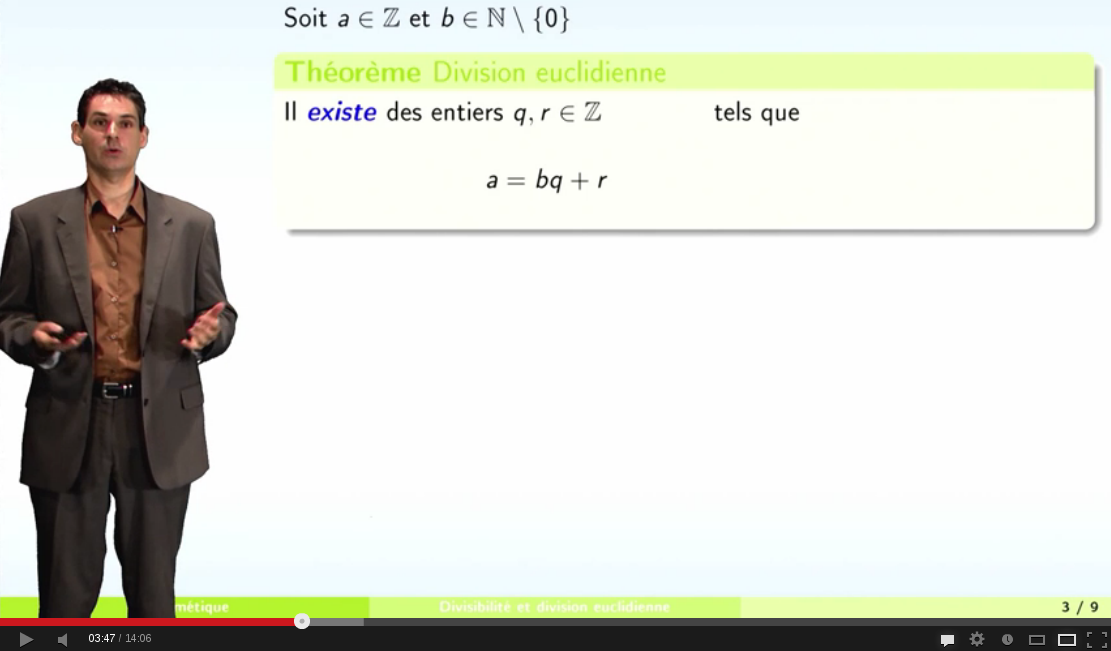
\includegraphics[scale=0.08]{Fig-crypto/img_video.png} &
\pause
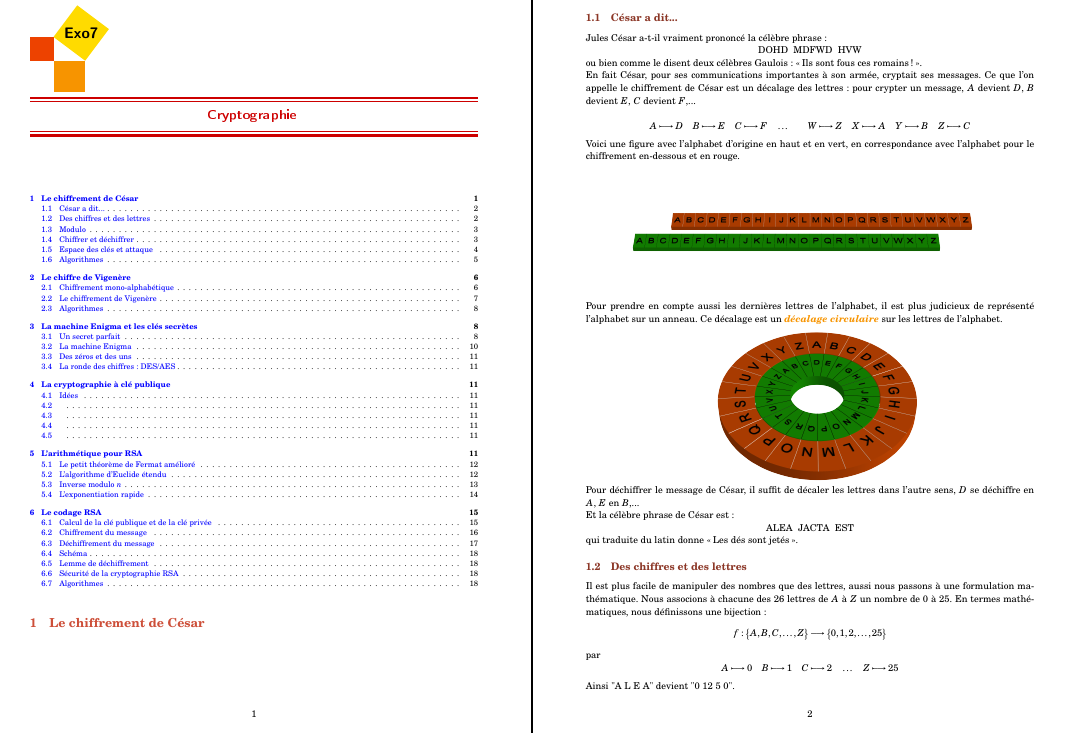
\includegraphics[scale=0.08]{Fig-crypto/img_cours.png} \\
\pause
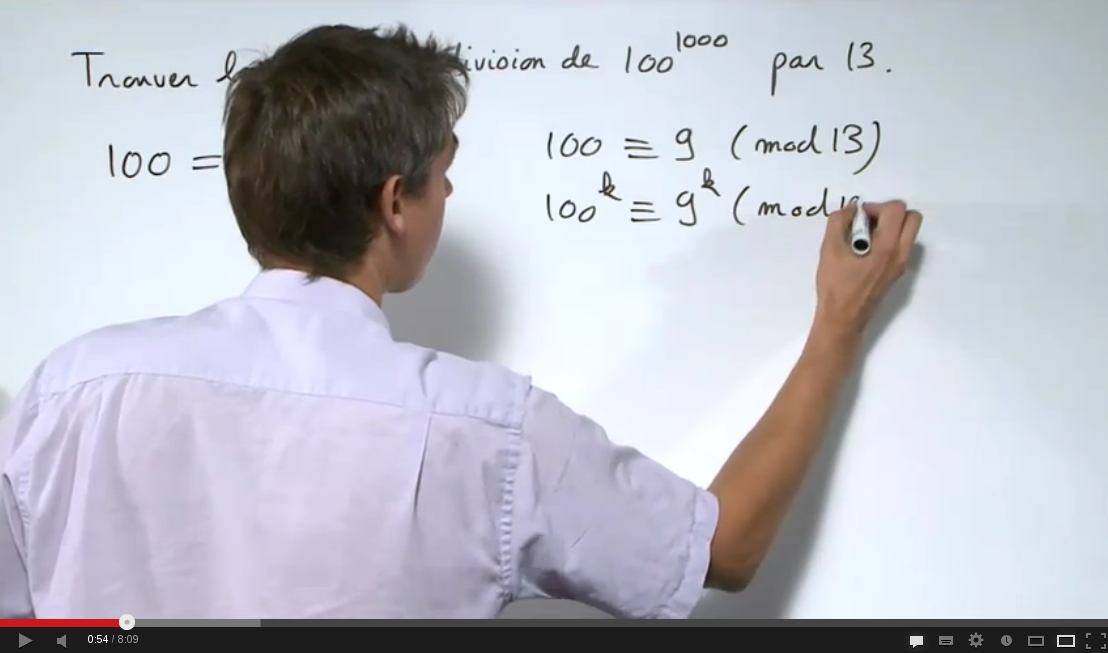
\includegraphics[scale=0.08]{Fig-crypto/img_exercice.png} &
\pause
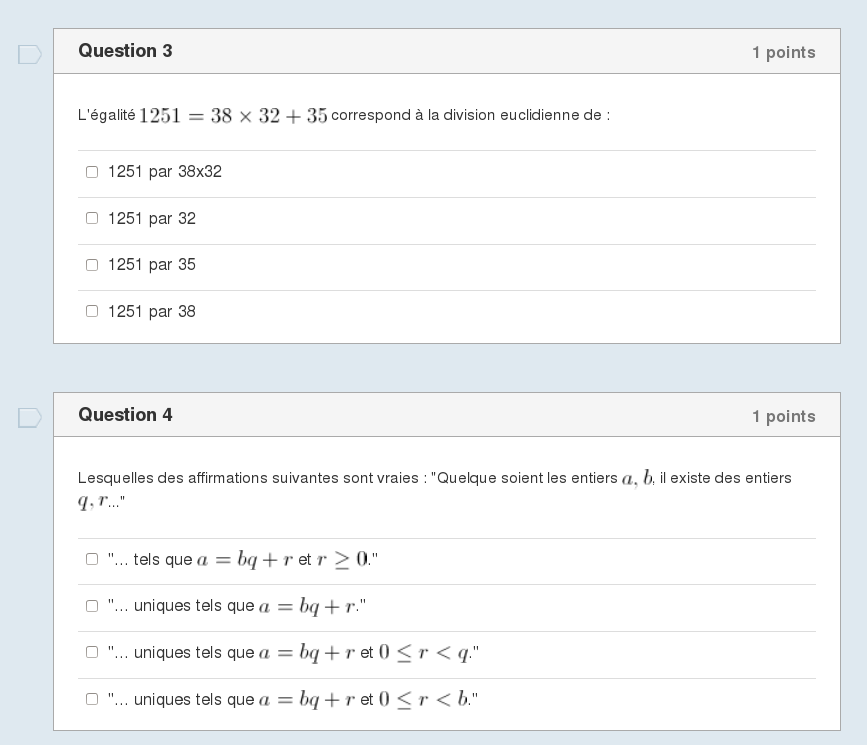
\includegraphics[scale=0.08]{Fig-crypto/img_qcm.png} \\ 
\end{tabular}


% \begin{center}
% \begin{minipage}{0.45\textwidth}
% \begin{itemize}[<+->]
%   \item Niveau : Licence première année
%   \item Des vidéos
%   \item Un cours complet en ligne
%   \item Des exercices corrigés
%   \item Des qcm chaque semaine  
%   \item Un forum de discussions
% \end{itemize}
% \end{minipage}
% \end{center}
\end{frame}

\end{document}
